\testCom
{%Номер задачи
	3.172
}
{%Условие
	условие
}
{%Дано
	дано
}
{%Найти
	найти
}
{%Решение
	%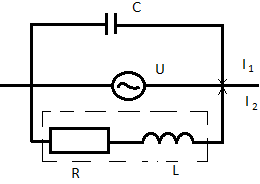
\includegraphics[height=50mm]{3_172.jpg}
	Правило Киргофа:\\
	$I_1 + I_2 - I_1$\\
	Нам надо найти разность фаз между U и I.\\
	$\tilde I_1 X_c = \tilde U$\\
	$\tilde I_2 (X_L + R) = \tilde U \Rightarrow \tilde I_1 = i \tilde U \omega c, \bar I_2 =\frac{\tilde U}{i \omega L + R}$\\
	разность фаз $= arg \tilde I - arg \tilde U = arg \tilde I - \omega t:$\\
	$\tilde I = \tilde I_1 + \tilde I_2 = \frac{\tilde U}{R^2 + \omega^2 L^2} (R + i(\omega c (R^2 + \omega^2 L^2) - \omega L))$\\
	$arg \tilde I = \omega t + \alpha,\alpha = \arctg \frac{\omega c (R^2 + \omega^2 L^2) - \omega L}{R}$\\
}

